\documentclass[12pt,a4paper,oneside,english]{book}


\usepackage[latin1]{inputenc}
\usepackage[T1]{fontenc}
\usepackage[english]{babel}
\usepackage{amsmath}
\usepackage{amsfonts}
\usepackage{amssymb}
\usepackage{graphicx}
\usepackage{subfig}
\usepackage{fancyhdr}
\usepackage{appendix}
\usepackage{hyphenat}
\usepackage{pdfpages}
\usepackage{natbib}
%\bibliographystyle{unsrtnat}
%\usepackage[
%backend=biber,
%style=alphabetic,
%sorting=ynt
%]{biblatex}
%\addbibresource{references.bib}



\usepackage{listings}
\usepackage{color}

\definecolor{dkgreen}{rgb}{0,0.6,0}
\definecolor{gray}{rgb}{0.5,0.5,0.5}
\definecolor{mauve}{rgb}{0.58,0,0.82}

\lstset{frame=tb,
  language=Java,
  aboveskip=3mm,
  belowskip=3mm,
  showstringspaces=false,
  columns=flexible,
  basicstyle={\small\ttfamily},
  numbers=none,
  numberstyle=\tiny\color{gray},
  keywordstyle=\color{blue},
  commentstyle=\color{dkgreen},
  stringstyle=\color{mauve},
  breaklines=true,
  breakatwhitespace=true,
  tabsize=3
}



\usepackage{array,multirow,makecell}
\newcolumntype{C}[1]{>{\arraybackslash}p{#1}}

\usepackage{enumitem}
\setlist{leftmargin=*,itemsep=0pt}

\usepackage{centernot}
\usepackage[linesnumbered,ruled,vlined,english,onelanguage]{algorithm2e}

\usepackage{quotchap}
\makeatletter
\renewcommand{\@makechapterhead}[1]{
 \chapterheadstartvskip
 {\size@chapter{\sectfont\raggedright
 {\chapnumfont
 \ifnum \c@secnumdepth >\m@ne
 \if@mainmatter\thechapter
 \fi\fi
 \par\nobreak}
 {\raggedright\advance\leftmargin10em\interlinepenalty\@M #1\par}}
 \nobreak\chapterheadendvskip}}
\makeatother
\renewcommand*{\chapterheadendvskip}{\vspace{2cm}}

\usepackage{geometry}
\geometry{hmargin=2.5cm,vmargin=2.5cm}

\pagestyle{fancyplain}
\lhead{\fancyplain{}{\nouppercase{\textit{\leftmark}}}}
\chead{\fancyplain{}{}}
\rhead{\fancyplain{}{}}
\lfoot{\fancyplain{}{}}
\cfoot{\fancyplain{}{}}
\rfoot{\fancyplain{\thepage}{\thepage}}
\renewcommand{\headrulewidth}{1pt}
\renewcommand{\footrulewidth}{1pt}

\renewcommand{\thesection}{\arabic{section}}

\usepackage{titlesec}
\titleformat{\paragraph}{\fontsize{11}{10}\bfseries}{\theparagraph}{1em}{}
\titlespacing*{\paragraph}{0pt}{10pt plus 2pt minus 0pt}{0pt plus 2pt minus 0pt}

\setcounter{secnumdepth}{4}
\setcounter{tocdepth}{4}

\usepackage{array}
\usepackage{multirow}
%\addto\captionsfrench{\def\tablename{\textsc{Tableau}}}

%\DefineBibliographyStrings{french}{urlseen = {},}

\setlength{\parskip}{8pt}
\usepackage{setspace}

\usepackage{url}

\usepackage{hyperref}
% Comment before printing to remove links' colors
\definecolor{darkblue}{rgb}{0.0, 0.0, 0.5}
\hypersetup{
 colorlinks,
 linktocpage=true,
 linkcolor={darkblue},
 citecolor={darkblue},
 urlcolor={blue}}

\sloppy

\author{You}
\title{Rapport de PFE}

\begin{document}
\pagenumbering{gobble}
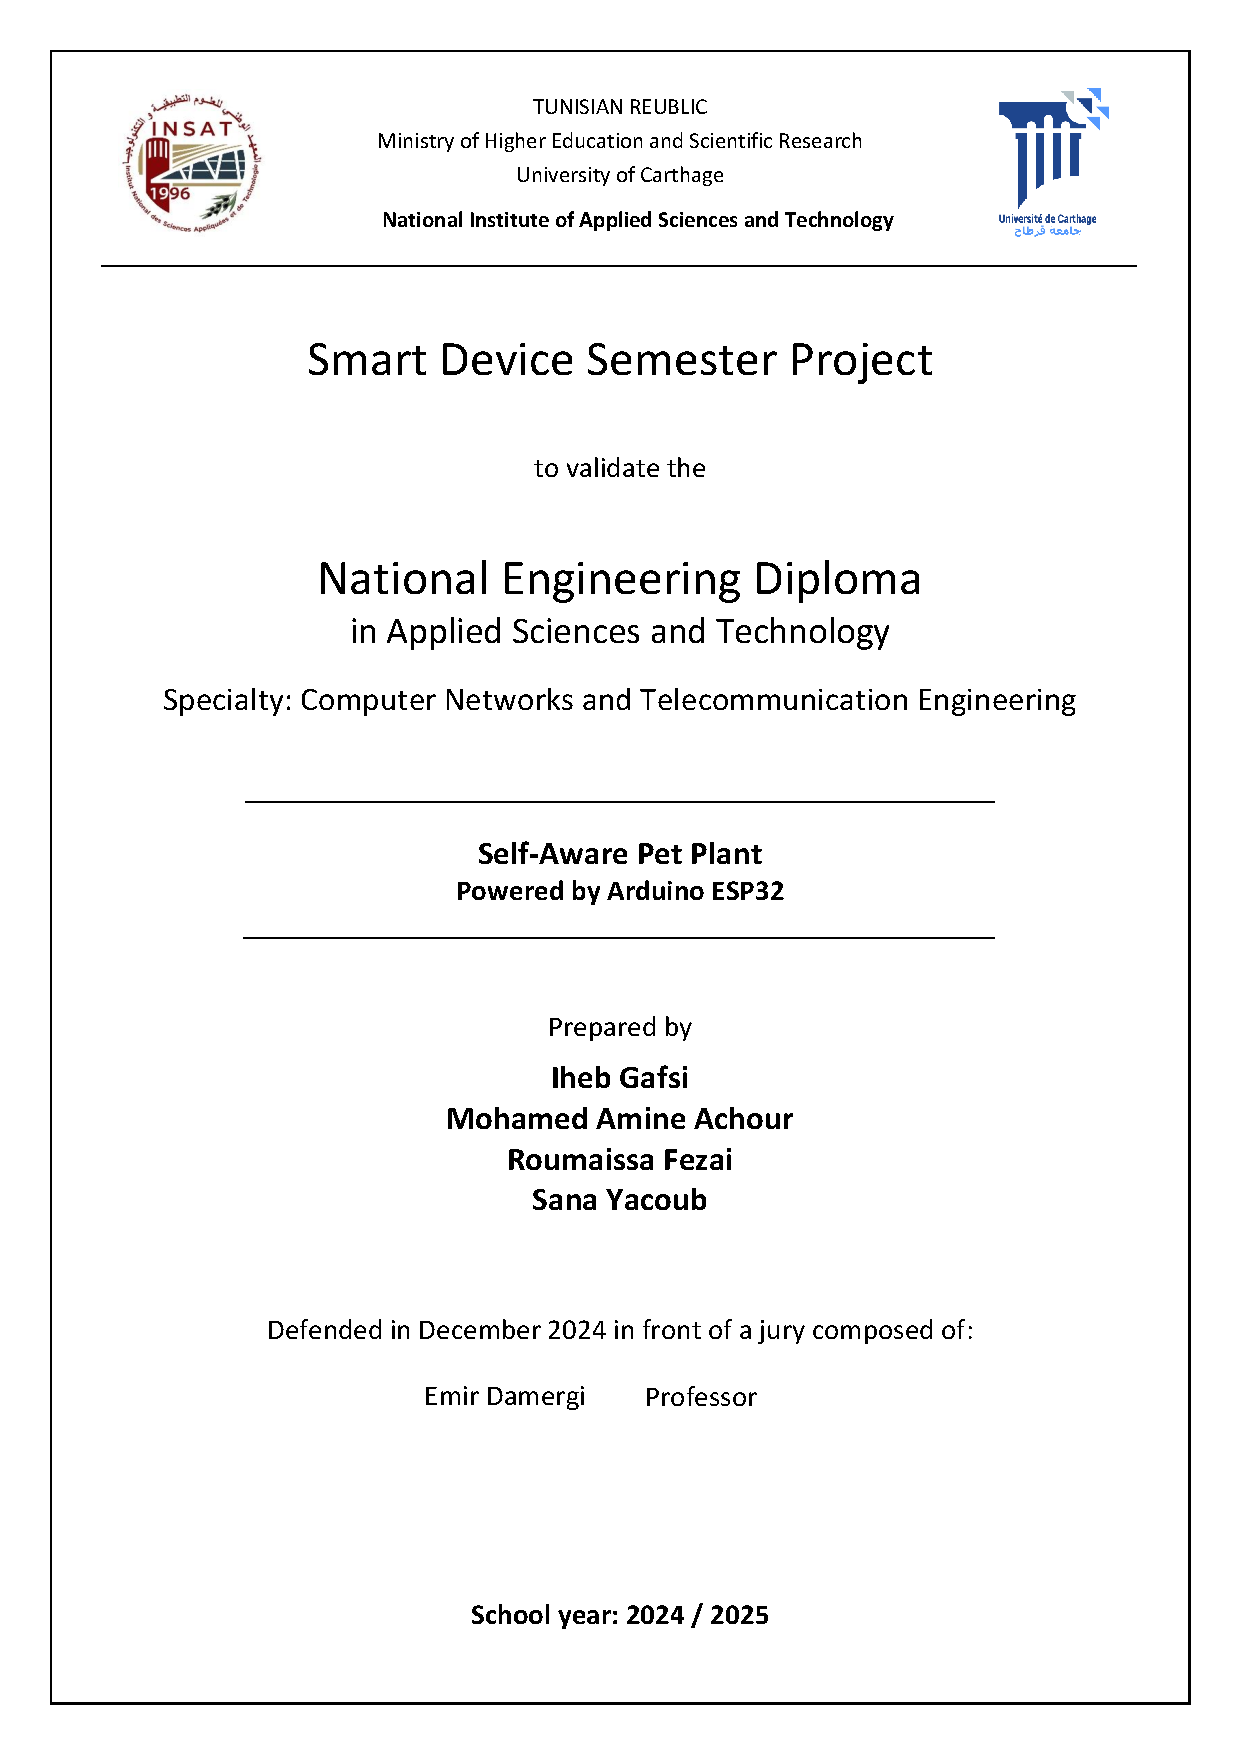
\includepdf[pages=-]{FrontPage.pdf}
\chapter*{Acknowledgments}
We would like to express our deepest gratitude to Professor Emir Damergi for his valuable guidance, encouragement, and insightful feedback throughout this project. His expertise and support have been instrumental in shaping our work and bringing this project to fruition.

We also extend our heartfelt thanks to the faculty and staff of the National Institute of Applied Sciences and Technology for providing us with the knowledge and resources necessary to complete this project successfully.

Additionally, we are grateful to our families and friends for their unwavering support, patience, and encouragement during the course of this project. Their motivation has been a constant source of inspiration for us.

Finally, we acknowledge the collaborative spirit and dedication of our team members, whose hard work and determination made the Self-Aware Pet Plant a reality.


\frontmatter
\chapter*{Abstract}
\normalsize{
    The Self-Aware Pet Plant is an IoT-based smart device, using the Arduino ESP32 microcontroller, which was designed to make plant care easier. This project leverages real-time environmental monitoring by integrating a temperature sensor and a humidity sensor to assess the plant's needs. This system uses the MQTT protocol for efficient data transmission in publishing temperature, humidity, and alert messages. Notifications, such as reminders to irrigate or notifications to move the plant, are generated based on set thresholds.

    The device seamlessly connects with a Wi-Fi network for continuous communication with an MQTT broker, providing users with actionable information that will help in maintaining optimal plant health. The incorporation of energy-efficient hardware, effective sensor data processing, and an advanced decision-making algorithm makes the Self-Aware Pet Plant function effectively under operational conditions.
    
    This project highlights the real application of IoT technologies, processing in real time, and environmental monitoring to improve everyday activities in accordance with interdisciplinary principles of Computer Networks and Telecommunication Engineering.
}

\medskip
{\noindent \textbf{Keywords: Smart device, Arduino ESP32, IoT, MQTT, environmental monitoring, plant care, temperature sensor, humidity sensor, real-time feedback, sustainable technology, Computer Networks and Telecommunication Engineering.} }

\spacing{1}
\tableofcontents{}
\newpage 
\listoffigures
\newpage 
\listoftables
\newpage
\spacing{1.4}
\chapter*{List of acronyms}
%\addcontentsline{toc}{chapter}{Liste des acronymes}
\markboth{List of acronyms}{}
\begin{itemize}
\item \textbf{IoT} Internet of Things
\item \textbf{ESP32} Espressif Systems' ESP32 microcontroller
\item \textbf{MQTT} Message Queuing Telemetry Transport
\item \textbf{Wi-Fi} Wireless Fidelity
\item \textbf{LM75} Temperature sensor
\item \textbf{DHT11} Digital temperature and humidity sensor
\item \textbf{DHT22} Digital temperature and humidity sensor
\item \textbf{BLE} Bluetooth Low Energy
\item \textbf{SRAM} Static Random-Access Memory
\item \textbf{PSRAM} Pseudo-Static Random-Access Memory
\item \textbf{ADC} Analog-to-Digital Converter
\item \textbf{O.S.} Overtemperature output
\item \textbf{VOCs} Volatile Organic Compounds
\item \textbf{PM2.5} Particulate Matter 2.5
\item \textbf{CO\textsubscript{2}} Carbon Dioxide
\item \textbf{NO\textsubscript{2}} Nitrogen Dioxide
\item \textbf{CO} Carbon Monoxide
\item \textbf{SO\textsubscript{2}} Sulfur Dioxide
\item \textbf{O\textsubscript{3}} Ozone
\item \textbf{PM10} Particulate Matter 10
\item \textbf{NH\textsubscript{3}} Ammonia
\item \textbf{H\textsubscript{2}S} Hydrogen Sulfide
\item \textbf{HCHO} Formaldehyde
\item \textbf{TVOC} Total Volatile Organic Compounds
\item \textbf{RH} Relative Humidity
\item \textbf{I2C} Inter-Integrated Circuit
\item \textbf{SPI} Serial Peripheral Interface
\item \textbf{UART} Universal Asynchronous Receiver-Transmitter
\item \textbf{LED} Light Emitting Diode
\item \textbf{PCB} Printed Circuit Board
\item \textbf{API} Application Programming Interface
\item \textbf{GUI} Graphical User Interface
\item \textbf{IDE} Integrated Development Environment
\end{itemize}

\mainmatter
%%\mtcaddchapter[Introduction g�n�rale] 
%\chapter*{Introduction}
%\addcontentsline{toc}{chapter}{Introduction}
%\markboth{Introduction}{}






\chapter{Introduction}
\section{Problem Statement}
In recent years, the use of technology to improve plant care has gained significant attention, particularly in the context of sustainable agriculture and smart home systems. Traditional methods of plant care rely heavily on human observation and manual intervention, which can lead to inefficient water usage, poor plant health management, and inconsistent care. Moreover, it can be challenging for individuals without expertise in horticulture to maintain optimal conditions for plant growth, particularly regarding temperature and humidity.

The problem arises from the lack of a reliable and automated system that can monitor and manage environmental conditions in real-time for plants. While there are existing solutions in the market that focus on general environmental monitoring, they often lack the capability to assess plant-specific needs and provide actionable insights for optimal care. Additionally, many of these systems are expensive and not easily accessible for all users.

The objective of this project is to design and implement an intelligent, low-cost, and easy-to-use solution that integrates Internet of Things (IoT) technologies to monitor the environmental parameters-specifically temperature and humidity-of a plant. This system will provide real-time feedback to the user, indicating when the plant requires watering, needs to be moved to a sunnier location, or when other care actions are necessary. The project leverages the Arduino ESP32 microcontroller, temperature and humidity sensors, and MQTT for communication, aiming to bridge the gap between manual plant care and fully automated systems.

By solving these challenges, the system aims to improve plant health management, reduce resource waste, and make plant care more accessible to a wider audience, contributing to a smarter and more sustainable environment.


\section{Objectives of the Project}
The primary objective of this project is to design and implement a self-aware plant monitoring system powered by the \texttt{Arduino ESP32} that can autonomously monitor the environmental conditions, such as temperature and humidity, and provide real-time feedback to users about their plant's needs. The specific objectives are:

\begin{itemize}
    \item \textbf{To develop a smart plant monitoring system} that can detect key environmental factors, including temperature and humidity, which are crucial for plant care.
    \item \textbf{To integrate IoT technologies} (Wi-Fi and MQTT) into the system, allowing for real-time data transmission and alerting the user when the plant requires care, such as watering or repositioning for better sunlight exposure.
    \item \textbf{To ensure system affordability and accessibility} by utilizing widely available and low-cost components (Arduino ESP32, LM75 temperature sensor, and a humidity sensor), making the system viable for everyday users.
    \item \textbf{To create an alert system} that provides actionable insights, such as warnings about high temperature, low humidity, or other conditions that could negatively impact plant health.
    \item \textbf{To enhance the user experience} by simplifying the plant care process through a mobile device or computer interface, enabling users to monitor their plants remotely and receive notifications.
    \item \textbf{To build a foundation for future improvements}, such as integrating additional sensors, incorporating machine learning for more accurate predictions, or expanding the system's capabilities to handle multiple plants.
\end{itemize}

\section{Importance of IoT in Plant Care}
The integration of Internet of Things (IoT) technology in plant care has revolutionized the way we interact with and manage plants. The traditional methods of plant care, which often rely on manual observation and human intervention, can be inefficient and inconsistent. With the advent of IoT, it is now possible to monitor and manage the environmental conditions that affect plant health in real-time, ensuring optimal care with minimal effort. The importance of IoT in plant care can be summarized in the following key points:

\begin{itemize}
    \item \textbf{Automation of Plant Care:} IoT devices can automate the monitoring of environmental parameters such as temperature, humidity, and soil moisture, reducing the need for constant human observation. This ensures that plants receive the correct care at all times, even in the absence of the plant owner.
    \item \textbf{Precision and Customization:} IoT sensors provide real-time data on plant conditions, allowing for precise control over environmental factors. This customization helps meet the specific needs of different plant species, improving plant health and growth rates.
    \item \textbf{Resource Efficiency:} By monitoring conditions such as soil moisture and temperature, IoT systems can optimize water and energy usage. This leads to more sustainable practices, reducing resource waste while maintaining plant health.
    \item \textbf{Remote Monitoring and Control:} IoT-enabled systems allow users to monitor their plants remotely via smartphones, computers, or other connected devices. This feature is especially beneficial for people who travel frequently or lack the time to care for plants in person.
    \item \textbf{Data-Driven Insights:} IoT systems generate valuable data that can be used to analyze plant growth patterns, predict optimal care routines, and even prevent potential issues before they arise. This data-driven approach provides a deeper understanding of plant needs and enhances care strategies.
    \item \textbf{Enhanced Accessibility:} IoT technology makes it easier for people, even those without expertise in horticulture, to successfully care for plants. The system can provide alerts and suggestions, reducing the complexity of plant care for beginners and improving the experience for experienced gardeners.
\end{itemize}

In conclusion, the importance of IoT in plant care lies in its ability to provide smarter, more efficient, and sustainable solutions for maintaining plant health. By utilizing IoT technology, plant care becomes more accessible, automated, and data-driven, benefiting both individual plant owners and larger-scale agricultural operations.

\chapter{Theoretical Study}
\section{Literature Review}
\subsection{Existing Smart Plant Care Solutions}
Among the works that have been presented to provide a solution for the care of ornamental plants planted in pots, we can mention the one carried out by Yuan et al. \citep{yuan2020iot}, who studied several of the factors affecting plant growth, proposing an IoT-based framework that allows scientists to collect data on environmental factors (such as temperature, light intensity, and CO2 concentration) in order to understand their impact on plant growth. One of the concerns about indoor plant care is addressed by Theparod et al. \citep{theparod2019iot}, who tried to supply the light needed for plants to grow by means of an IoT device with light emitting diodes. Another need plants have is water. Ting et al. \citep{ting2020irrigation} presented a system to control plant irrigation based on environmental parameters, such as soil moisture, air humidity, environmental temperature, and light intensity. Banda-Chavez et al. \citep{banda2018intelligent} monitored soil moisture and environmental temperature factors and, depending on the values of these parameters, activated or not a pump to wet the soil of the plants. Likewise, Azhar et al. \citep{azhar2017controlling} provided the necessary water and fertiliser to the plants, according to the detected values of environmental temperature and humidity, as well as the soil moisture and temperature. However, none of the aforementioned papers presenting a contribution to plant care that combines water and fertilizer supply, lighting and alert the users when the indoor air quality is poor or dangerous for their health.

Potted ornamental plants can be used to decontaminate indoor environments, since they can help to reduce indoor pollution levels, though their care may be a challenge for their owners. In some cases, indoor pollution levels can be up to 100 times higher than outdoor pollution levels \citep{johannessen2020embedded}. Indoor pollution can be caused by the entry of vehicles either to load or unload goods in factories, workshops, or warehouses, or simply to park them in garages when these are inside homes \citep{brunel2019two}. One of the fields of application of IoTS is the monitoring of the concentration levels of pollutant gases using sensors \citep{guerrero2023development,gezici2022systematic,guerrero2023agile} and, as mentioned above, one of the practices that have been implemented to help decontaminate indoor air and improve its quality is the use of ornamental plants \citep{chowdhury2021effects,barra2022artificial,kumar2022probabilistic}. These two practices, i.e., technology-based surveillance and the use of ornamental plants, can be combined and complement each other. This allows people who are (working or living) in that indoor space to breathe better quality air, thanks to the production of oxygen and the reduction of pollutants, benefits provided by the photosynthesis process of the plants, with the added advantage of hardly having to worry about their care, if their owners so wish.

According to the papers retrieved in our study of the state of the art, works proposing solutions for the care of potted plants and those proposing systems for pollution monitoring are divorced. Nonetheless, some authors, such as Guerrero-Ulloa et al. \citep{guerrero2020smartmedicine} propose a system that not only monitors and alerts about pollution levels but also tries to decrease pollution by turning on fans and opening windows automatically. Therefore, our proposal, which is described in the following section, tries to overcome the limitations of the analysed systems. P4L allows not only the care of potted plants, providing them with sufficient water and fertiliser, but also the monitoring of the levels of pollutant gases in the environment. In addition, P4L will be able to send notifications to the user via its mobile application, according to the concentration levels of pollutant gases in the environment and inform the user about the state of the plant.

Moreover, the indoor of such standardised equipment is the accountability that manufacturers can provide for periodic calibration and validation, they may not be suitable for long-term monitoring (8, 12 or 24/7, uninterrupted), as they are limited to the time of their battery life \citep{yang2021long}. The cost of such a device increases if you add the cost of a system for the care of indoor potted plants. This is why we present a low-cost solution that covers these two fields (automated plant care and pollutant gas monitoring), and provides better quality air to breathe, which will benefit the health of the people in the space or environment in which the system we propose is placed.


\subsection{Overview of IoT Applications in Environmental Monitoring}
The Internet of Things (IoT) has become an essential technology for environmental monitoring, allowing for real-time data collection and analysis of environmental parameters across various domains. In recent years, the application of IoT in environmental monitoring has expanded to several critical areas, including agriculture, air quality control, water management, and climate change monitoring. The integration of IoT sensors and devices in these areas has enabled better decision-making, resource management, and enhanced sustainability.

Some of the key IoT applications in environmental monitoring include:

\begin{itemize}
    \item \textbf{Agricultural Monitoring:} IoT technology plays a pivotal role in modern agriculture by providing farmers with the ability to monitor soil conditions, weather, temperature, and humidity levels. Smart sensors placed in the soil or attached to plants allow for real-time data collection, enabling farmers to optimize irrigation, manage water usage, and apply fertilizers or pesticides in a targeted manner. This leads to improved crop yields, reduced resource consumption, and increased sustainability.
    
    \item \textbf{Air Quality Monitoring:} IoT-based air quality monitoring systems help in tracking the concentration of pollutants, such as carbon dioxide (CO\textsubscript{2}), nitrogen dioxide (NO\textsubscript{2}), particulate matter (PM2.5), and volatile organic compounds (VOCs) in the atmosphere. These systems provide real-time data that can be used to detect air pollution and assess the effectiveness of air quality control measures. IoT sensors are also crucial for urban planning and improving the health and safety of city environments.
    
    \item \textbf{Water Quality Monitoring:} IoT applications are increasingly used to monitor the quality of water bodies, including rivers, lakes, and reservoirs. Sensors placed in or around water sources collect data on parameters such as pH levels, temperature, turbidity, and chemical contamination. Real-time data from IoT systems allows for early detection of water pollution, better management of water resources, and quicker response to environmental hazards.
    
    \item \textbf{Climate Change Monitoring:} Climate change is one of the most pressing global challenges, and IoT-based monitoring systems are playing a vital role in collecting data to understand climate patterns and predict future trends. IoT sensors installed in various locations can measure temperature, humidity, wind speed, and other environmental variables to track shifts in weather patterns and help scientists and policymakers develop mitigation strategies.
    
    \item \textbf{Energy Consumption Monitoring:} IoT devices are also applied in monitoring and managing energy usage in homes, industries, and cities. Smart meters and sensors provide data on energy consumption, allowing for efficient management of electricity, water, and heating resources. By optimizing energy consumption, IoT systems contribute to reducing carbon footprints and promoting sustainability.
\end{itemize}

In all these applications, IoT technology provides the ability to gather real-time data, which is crucial for monitoring environmental changes and making informed decisions. The data generated by IoT devices can be analyzed to identify trends, predict potential environmental risks, and implement timely interventions. As the need for more sustainable and efficient environmental management practices grows, the role of IoT in environmental monitoring will continue to expand, offering new opportunities for innovation and impact.

\section{System Design Overview}
\subsection{Concept of Smart Plants and IoT}
The concept of smart plants, empowered by Internet of Things (IoT) technology, refers to the integration of sensors, actuators, and connected devices to monitor and manage plant care more efficiently. These "smart" plants are capable of collecting real-time data on environmental factors such as temperature, humidity, soil moisture, and light levels, which are critical for their growth and health. IoT-based systems use this data to automate the care process, sending alerts or taking actions like watering or adjusting light exposure based on the plant's needs.
Smart plants utilize a combination of hardware and software components to function autonomously or with minimal human intervention. The key components of a smart plant system include:
\begin{itemize}
    \item \textbf{Sensors:} Sensors are the core of any smart plant system, collecting data from the plant's environment. Common sensors used in smart plant systems include temperature sensors (such as LM75), humidity sensors, soil moisture sensors, and light sensors. These sensors provide real-time measurements, allowing the system to assess the plant's current conditions.
    
    \item \textbf{Actuators:} Actuators perform specific actions based on the data received from the sensors. For example, a smart irrigation system can automatically water the plant when the soil moisture level drops below a set threshold. Actuators can also control other aspects of plant care, such as adjusting light exposure or activating fans to regulate temperature.
    
    \item \textbf{Microcontroller/Controller Unit:} The microcontroller, such as the \texttt{Arduino ESP32}, serves as the brain of the smart plant system. It processes data from the sensors and makes decisions based on predefined rules or algorithms. The microcontroller also manages communication with other devices, such as mobile phones or cloud platforms, to send notifications or trigger actions in real-time.
    
    \item \textbf{Connectivity:} IoT technology relies on connectivity to enable remote monitoring and control. In smart plant systems, Wi-Fi or Bluetooth is typically used to connect the plant to a cloud service, mobile app, or other devices. This connectivity allows users to monitor their plants remotely, receive alerts, and make changes to the plant's care routine from anywhere in the world.
    
    \item \textbf{Data Analytics:} The data collected by sensors is analyzed to derive meaningful insights. This data can be used to predict future plant care needs, adjust environmental conditions, or even detect early signs of stress or disease. Data analytics plays a key role in optimizing plant care and ensuring plant health in a sustainable manner.
\end{itemize}
The use of IoT in smart plant systems enables the automation of daily plant care routines, which is particularly beneficial for people who may not have the time or expertise to care for plants. These systems can provide real-time alerts, such as when the plant needs watering, when it should be moved to a different location for more sunlight, or when the humidity or temperature falls outside the optimal range for plant health.
Additionally, smart plants contribute to sustainability by optimizing resource usage. For example, IoT-enabled systems can monitor and control water usage, ensuring that plants are watered only when necessary, which helps conserve water in areas where it is scarce.
In summary, the concept of smart plants and IoT revolves around creating an intelligent, connected system that helps improve plant care through automation, remote monitoring, and data-driven decision-making. By leveraging IoT technology, plant owners can ensure the health and well-being of their plants while reducing manual effort and resource waste.

\begin{figure}[!h]
    \centering
    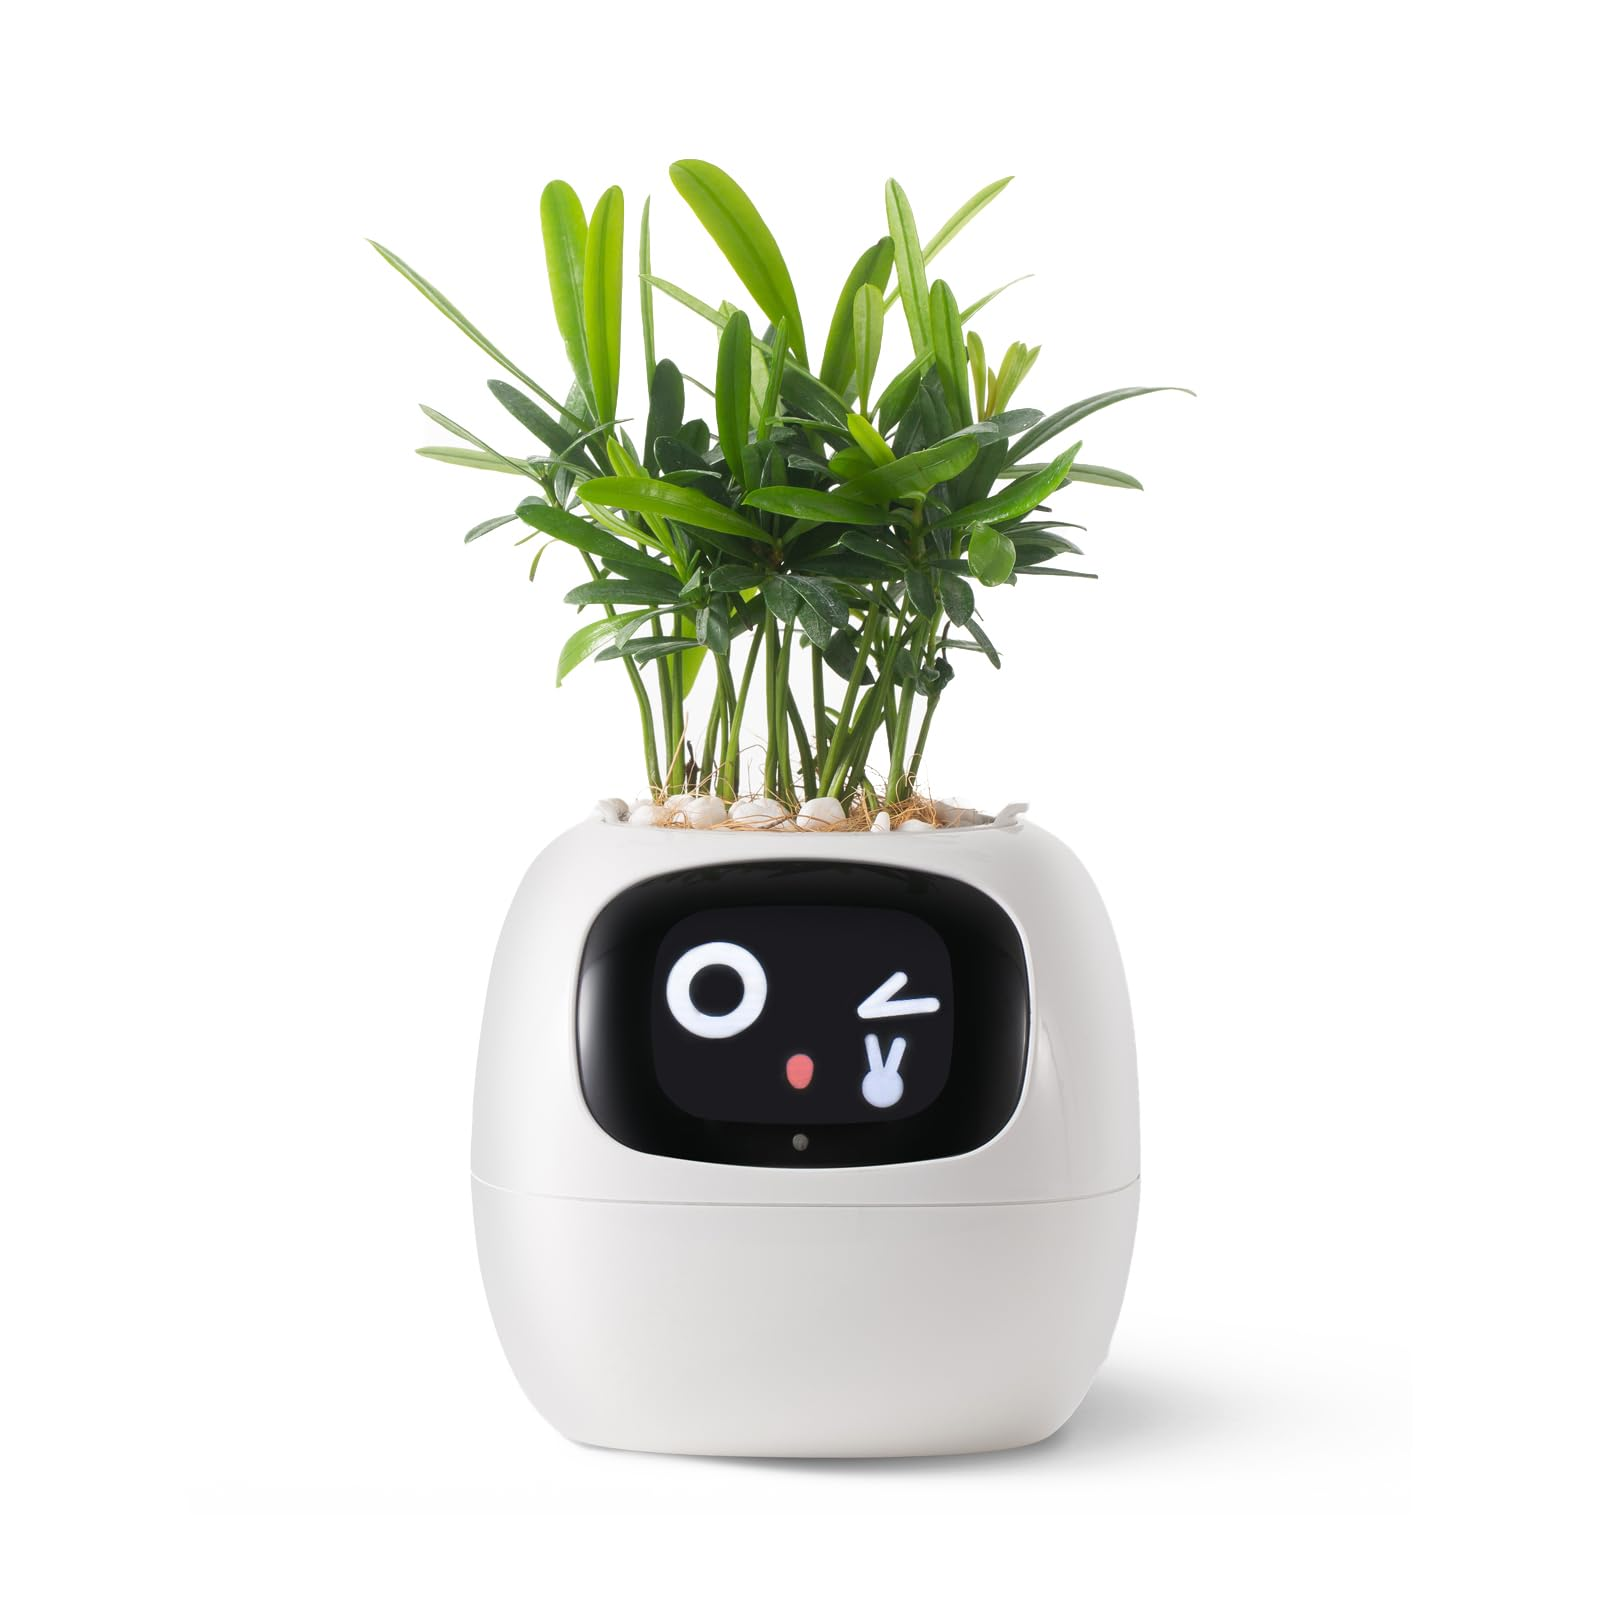
\includegraphics[width=0.3\textwidth]{images/petplant.jpg}
    \caption{Concept of Smart Plant Care System}
    \label{fig:smartpetplant}
\end{figure}




\subsection{Role of Temperature and Humidity in Plant Care}

Temperature and humidity are two of the most important environmental factors that influence plant health and growth. Plants have specific temperature and humidity ranges within which they thrive, and any deviations from these optimal conditions can lead to stress, inhibited growth, or even plant death. Understanding and controlling these factors is essential for ensuring healthy plant development, especially in controlled environments such as homes, greenhouses, or urban spaces.

\subsubsection{Importance of Temperature}

Temperature affects numerous physiological processes in plants, including photosynthesis, respiration, and transpiration. Each plant species has an ideal temperature range that supports its metabolic processes. If the temperature falls outside this range, the plant may not perform these functions efficiently, leading to reduced growth and potential damage.

\begin{itemize}
    \item \textbf{Photosynthesis and Respiration:} At temperatures that are too high or too low, plants may not be able to photosynthesize effectively, reducing their energy production and growth rate. Similarly, respiration processes can be slowed or disrupted, limiting the plant's ability to convert stored energy into growth.
    \item \textbf{Dormancy and Growth:} Temperature also determines when a plant enters dormancy and when it resumes growth. Many plants require a period of cool temperatures to enter dormancy, while others need warmth to trigger new growth in the spring.
    \item \textbf{Optimal Growth Range:} Each plant species has a specific optimal temperature range, typically between 15°C and 25°C, within which it grows most efficiently. Extreme temperatures, either hot or cold, can cause stress, wilting, or death, making it critical to monitor and regulate temperature conditions.
\end{itemize}




\subsection{Interaction Between Temperature and Humidity}

Temperature and humidity are closely interrelated, and their combined effects on plant health must be considered together. The rate of transpiration, for example, is higher at higher temperatures and lower humidity, leading to faster water loss and potential dehydration. Conversely, low temperatures coupled with high humidity can lead to condensation on plant surfaces, fostering the growth of pathogens.

In some cases, adjustments to one parameter (e.g., reducing temperature) can help mitigate the effects of an unfavorable humidity level, and vice versa. For instance, reducing the temperature of a room may help lower the rate of transpiration and reduce water loss in a plant suffering from low humidity.

\subsection{IoT's Role in Monitoring Temperature and Humidity}

With the integration of IoT technology, monitoring temperature and humidity has become more accessible and automated. IoT sensors allow for continuous tracking of environmental conditions, providing real-time data that can be used to adjust care routines accordingly. When temperature or humidity levels fall outside the optimal range, IoT-based systems can send alerts or trigger automated actions, such as activating a humidifier, adjusting the thermostat, or watering the plant.

By using IoT devices to monitor and adjust temperature and humidity levels, plant owners can ensure their plants are always in the best possible conditions, leading to healthier growth and a more sustainable care routine.







\subsection{MQTT Protocol and Its Use in IoT}
The MQTT protocol defines two kinds of network entities: a message broker and a number of clients. One MQTT broker is a server that receives all messages from the clients and then routes the messages to the appropriate destination clients. An MQTT client is any device (from a micro controller up to a fully-fledged server) that runs an MQTT library and connects to an MQTT broker over a network.

Information is organized in a hierarchy of topics. When a publisher has a new item of data to distribute, it sends a control message with the data to the connected broker. The broker then distributes the information to any clients that have subscribed to that topic. The publisher does not require to keep any information on the numbers and locations of subscribers and the subscribers in turn do not need to be configured with any data on the publishers.

In case a broker receives a message on a topic without active subscribers, the broker will discard the message unless the publisher of the message designated the message as a retained message. A retained message is a regular MQTT message, which has the retained flag set to true. The broker stores the last retained message and the corresponding QoS for the selected topic. Every client that subscribes to a topic pattern which matches the topic of the retained message receives the retained message instantly after they subscribe. The broker stores only one retained message per topic. This allows new subscribers to a topic to receive the most current value rather than waiting for the next update from a publisher.

When a publishing client first connects to the broker, it can set up a default message to be sent to subscribers if the broker detects that the publishing client has unexpectedly disconnected from the broker.

Clients interact only with a broker, but a system can have several broker servers, which may exchange data on the basis of their current subscribers' topics.

A minimal MQTT control message can be as little as two bytes of data. If needed a control message can carry nearly 256 megabytes of data. There are fourteen defined message types used to connect and disconnect a client from a broker, to publish data, to acknowledge receipt of data and to supervise the connection between client and server.

MQTT is based on the TCP protocol for the transport of data. A variant, MQTT-SN, is used over other transports such as UDP or Bluetooth.

MQTT sends the connection credentials in plain text format and does not have any measures for security or authentication. This can be provided by using TLS to encrypt and protect the transferred information against interception, modification or forgery.

The default unencrypted MQTT port is 1883. The encrypted port is 8883.




\section{Theoretical Analysis of Components}
\subsection{Arduino ESP32 Capabilities}
The Arduino Nano ESP32 is a compact development board that integrates the ESP32-S3 microcontroller, offering enhanced capabilities for various applications. This microcontroller features a dual-core 32-bit Xtensa LX7 processor with a floating-point unit, operating at up to 240 MHz, providing robust processing power for complex tasks \citep{arduino2023}.

In terms of memory, the ESP32-S3 includes 512 KB of SRAM and 8 MB of external PSRAM, accommodating the demands of memory-intensive applications \citep{arduino2023}.

Connectivity is a key strength of the Arduino Nano ESP32, supporting both Wi-Fi and Bluetooth Low Energy (BLE) standards. This dual connectivity enables seamless integration into Internet of Things (IoT) ecosystems, facilitating communication with a wide range of devices and networks \citep{arduino2023}.

The board is equipped with a variety of input/output options, including multiple digital I/O pins, analog inputs, and communication interfaces such as SPI, I2C, and UART. These features make it versatile for interfacing with sensors, actuators, and other peripherals \citep{arduino2023}.

Additionally, the Arduino Nano ESP32 supports advanced features like capacitive touch sensing, making it suitable for interactive applications \citep{arduino2023}.

Overall, the Arduino Nano ESP32 combines powerful processing capabilities, extensive connectivity options, and a rich set of features, making it an excellent choice for developing a wide range of IoT and embedded systems projects \citep{arduino2023}.


\subsection{Temperature Sensors: LM75}
The LM75 is a highly accurate digital temperature sensor designed for a variety of applications, from thermal monitoring in base stations to electronic test equipment. It uses a delta-sigma analog-to-digital converter (ADC) to convert temperature readings into a 9-bit digital output, which offers an accuracy of $\pm 2 ^\circ C$ from $-25^\circ C$ to $100^\circ C$, and $\pm 3^\circ C$ from $-55^\circ C$ to $125^\circ C$ \citep{tiLM75a}. This temperature sensor operates with a supply voltage ranging from 2.7 V to 5.5 V, making it versatile for different electronic systems \citep{tiLM75a}. The LM75 communicates over the I2C interface, allowing for up to eight devices to share the same bus, which simplifies integration into complex systems \citep{tiLM75a}. With a typical operating current of 280 $\mu A$ and a low-power shutdown mode consuming only 4 $\mu A$, the LM75 is energy-efficient, making it ideal for battery-powered devices or systems requiring low power consumption \citep{tiLM75a}. Moreover, it features a programmable overtemperature output (O.S.) with user-defined temperature limits and hysteresis, enhancing its ability to act as an alert system for abnormal temperature conditions \citep{tiLM75a,harvardTempMon}. This feature is particularly useful in applications such as thermal management in personal computers, office electronics, and even thermal monitoring in critical infrastructure systems \citep{universityThermal}.


\subsection{Humidity Sensors: Working Principles for Plant Care}

In the context of plant care, humidity sensors play a critical role in monitoring environmental conditions that directly affect plant health. These sensors help in regulating irrigation systems, ensuring that the plants receive the appropriate amount of moisture for optimal growth. The working principles of these sensors vary, with each type offering distinct advantages depending on the application and environment.

\subsubsection{Capacitive Humidity Sensors}

Capacitive humidity sensors operate by measuring changes in the dielectric constant of a material (typically a polymer) as it absorbs water vapor. This change in capacitance is directly related to the relative humidity of the environment. In the context of plant care, capacitive sensors are widely used because of their accuracy, low power consumption, and longevity, making them suitable for continuous environmental monitoring in IoT-based plant care systems \cite{yuan2020iot}. These sensors are also less affected by contaminants, which is essential in an agricultural or indoor setting where soil and dust can interfere with other types of sensors.

\subsubsection{Resistive Humidity Sensors}

Resistive humidity sensors function by detecting changes in the electrical resistance of a material as it absorbs moisture. Typically, these sensors use conductive polymers or salts that change resistance with humidity. Though resistive sensors are generally less accurate than capacitive sensors, they are cost-effective and can be used for less critical applications where high accuracy is not as essential \cite{theparod2019iot}. In the context of the Self-Aware Pet Plant project, resistive sensors can be used as part of a simple irrigation control system to monitor soil moisture levels, triggering water pumps when the soil is too dry.

\subsubsection{Digital Humidity Sensors}

Digital humidity sensors, such as the DHT11 and DHT22, combine temperature and humidity sensing in a single device, offering both high accuracy and ease of integration with microcontroller platforms like the Arduino ESP32. These sensors provide a digital output, making them ideal for use in automated systems where the data needs to be processed quickly and accurately. In the Self-Aware Pet Plant project, digital sensors like these can be connected to the ESP32 to monitor both temperature and humidity levels in real-time, adjusting the environment to ensure optimal conditions for plant growth \cite{ting2020irrigation}.

\subsubsection{Thermohygrometers and Advanced Systems}

Advanced systems, such as thermohygrometers, measure both temperature and humidity to provide a comprehensive view of the environmental conditions. These sensors are typically used in more precise and scientific applications, including monitoring the climate in greenhouses or research environments. In a project like the Self-Aware Pet Plant, combining temperature and humidity data can enable more advanced decision-making for plant care, including controlling fans for temperature regulation and adjusting irrigation systems based on a combination of humidity and temperature readings \cite{banda2020smart}.

By understanding the working principles of various humidity sensors, the Self-Aware Pet Plant project aims to integrate these technologies into an efficient and cost-effective solution for plant care. These sensors will help in creating a dynamic environment where moisture levels are carefully monitored and adjusted, promoting healthier and more resilient plants.


\chapter{Practical Approach}
\section{System Architecture and Implementation}
\subsection{Overview of the Physical System}
In this system we 
\subsection{Hardware Components}
\subsubsection{Arduino ESP32}
\subsubsection{LM75 Temperature Sensor}
\subsubsection{Humidity Sensor and Power Supply}
\subsection{Software Implementation}
\subsubsection{Wi-Fi Setup and Connection}
\subsubsection{MQTT Communication Setup}

\section{Practical Setup and Functionality}
\subsection{Circuit Design and Connections}
\subsection{Sensor Data Acquisition (Temperature \& Humidity)}
\subsection{Logic for Alerts (Based on Thresholds)}
\subsection{Data Transmission Using MQTT}

\section{Expected Outcomes and Practical Implications}
\subsection{Behavior of the System (Temperature, Humidity, Alerts)}
The system monitors temperature and humidity in real-time to ensure optimal conditions for plant care. Based on sensor data, it generates alerts to inform the user when action is needed.

\subsubsection{Temperature Behavior}
The system continuously tracks temperature. If the temperature exceeds a threshold (e.g., 30$^\circ$C) or drops below a critical limit (e.g., 15$^\circ$C), an alert is sent. The system may recommend moving the plant to a more suitable environment.

\subsubsection{Humidity Behavior}
Humidity is monitored to ensure it stays within an ideal range (40\%-60\%). Alerts are triggered if the humidity is too low (e.g., below 20\%) or too high (e.g., above 80\%). The system suggests watering the plant or adjusting humidity levels accordingly.

\subsubsection{Alert System}
The system generates alerts for critical conditions:
\begin{itemize}
    \item \textbf{High Temperature}: Above 40$^\circ$C - suggests moving the plant.
    \item \textbf{Low Temperature}: Below 15$^\circ$C - suggests relocating the plant.
    \item \textbf{Low Humidity}: Below 20\% - recommends watering.
    \item \textbf{High Humidity}: Above 80\% - advises reducing watering or improving ventilation.
\end{itemize}

\subsubsection{Practical Implications}
The system automates plant care by providing real-time alerts and recommendations. It helps optimize resource use, supports plant health, and reduces manual monitoring.

\subsection{Future Enhancements}
We plan to enhance the system by adding additional sensors, such as light sensors, soil moisture sensors, and air quality sensors. These enhancements will provide a more comprehensive view of the plant's environment and enable more precise care recommendations. We will also add better screen that handles showing emojis properly.

\chapter{Conclusion}
\section{Summary of Achievements}
\section{Practical Contributions of the Project}
\section{Future Work and Improvements}















\renewcommand{\bibname}{References}
\renewcommand{\bibsection}{\chapter{\bibname}}
\bibliographystyle{unsrtnat}
\bibliography{references.bib}
\newpage
%\printbibliography



\section*{Conclusion}

\chapter*{Conclusion and perspectives}
\addcontentsline{toc}{chapter}{Conclusion and perspectives}
\markboth{Conclusion and perspectives}{}

\begin{appendix}
\chapter{Appendix}
\section{Circuit Diagrams}
\begin{figure}[!h]
\centering
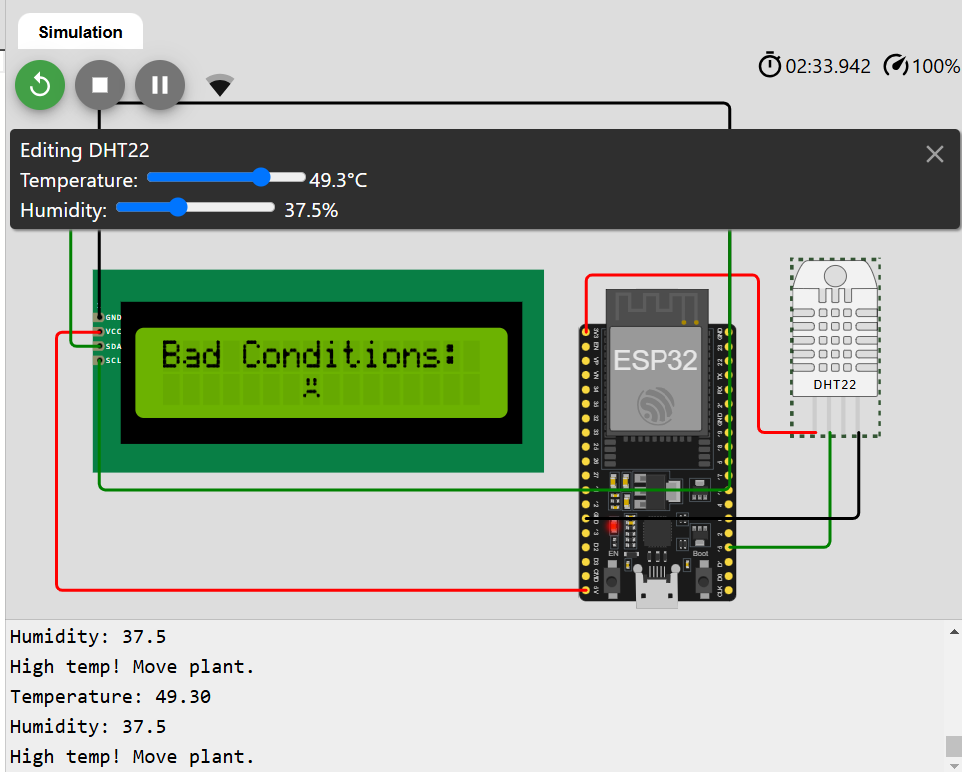
\includegraphics[width=0.6\textwidth]{images/badcondition.png}\label{fig:badconditionn}
\caption{This is the functioning system circuit when the plat is in a bad condition}
\label{fig:exemple1}
\end{figure}

\begin{figure}[!h]
    \centering
    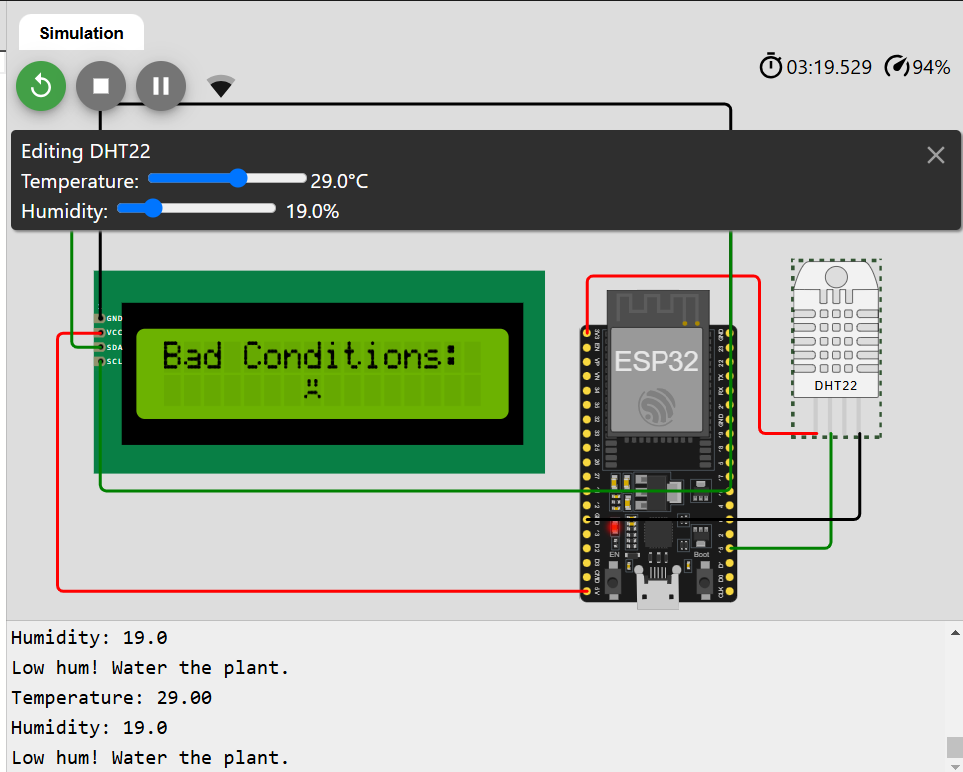
\includegraphics[width=0.6\textwidth]{images/badcondition2.png}\label{fig:badconditionn2}
    \caption{This is another example of the functioning system circuit when the plat is in a bad condition}
    \label{fig:exemple1}
\end{figure}

\section{Source Code}
\begin{lstlisting}
    #include <WiFi.h>
#include <PubSubClient.h>
#include <Wire.h>

#define LM75_ADDRESS 0x48
const char* ssid = "Infinix HOT 30";
const char* password = "roumaisaa";
const char* mqttServer = "broker.emqx.io";
const int mqttPort = 1883;
const char* mqttClient = "client121";
const char* TopicHum = "/projet/humidity";
const char* TopicTemp = "/projet/temperature";
const char* TopicAlert= "/projet/alerts"; 
WiFiClient espClient;
PubSubClient client(espClient);
void callback(char* topic, byte* payload, unsigned int length){};
void Read2Bytes(uint8_t RegAddr, uint8_t &highbyte, uint8_t &lowbyte) {
  Wire.beginTransmission(LM75_ADDRESS);
  Wire.write(RegAddr);
  Wire.endTransmission();
  
  Wire.requestFrom(LM75_ADDRESS, 2);
  
  if (Wire.available() == 2) {
    highbyte = Wire.read();
    lowbyte = Wire.read();  
  }
}
float CalculateTemperature(uint8_t highbyte, uint8_t lowbyte) {
  int16_t tempData = (highbyte << 8 | lowbyte);
  tempData >>= 5;
  if (tempData & 0x0400) {  
    tempData |= 0xF800; 
  }
  float temperature = tempData * 0.125;

  return temperature;
}


void Setup_WiFi() {
    WiFi.begin(ssid, password);
    while (WiFi.status() != WL_CONNECTED) {
        Serial.println("Connexion au WiFi...");
        delay(500);
    }
    Serial.println("ConnectE au WiFi");
}
void setup_MQTT() {
    client.setServer(mqttServer, mqttPort);
    client.setCallback(callback);
    while (!client.connected()) {
        if (client.connect(mqttClient)) {
            Serial.println("ConnectE au broker MQTT");
            client.subscribe(TopicTemp);
            client.subscribe(TopicHum);
            client.subscribe(TopicAlert);
        } else {
            Serial.println("Echec de connexion au broker MQTT. Nouvelle tentative...");
            delay(2000);
        }
    }
}


void setup(){
    Serial.begin(115200);
    Wire.begin();
    Setup_WiFi();
    setup_MQTT(); 
    
}

void loop() { 
   uint8_t highbyte, lowbyte;
   Read2Bytes(0x00, highbyte, lowbyte);
   float temperature = CalculateTemperature(highbyte, lowbyte);
  delay(1000);
    if (!client.connected()) {
        setup_MQTT();
    }
    client.loop();
    char buff[10];
    snprintf(buff, sizeof(buff), "%.2f",temperature );
    client.publish(TopicTemp,buff);
    int hum=40;
    char Hum[10];
    snprintf(Hum, sizeof(Hum), "%.2f", hum);
    client.publish(TopicHum, Hum);
    
    Serial.println("DonnEes de tempErature envoyEes  : " + String(buff));
    Serial.println("DonnEes de humidite envoyEes  : " + String(Hum));
    Serial.println("---");
    String alertMsg = "";
    if (temperature > 40 && hum < 20) {
    alertMsg = "High temperature & low humidty! Water & move plant. ";
    }    else if (temperature > 30 && hum > 80) {
    alertMsg = " High temperature & high  humidty! less water and move the plant";
    }
    else if (temperature > 30) {
    alertMsg = "High temperature! Move plant";
   } else if (hum < 20){
    alertMsg = "Low humidity! Water the plant";
   } else if (hum> 80) {
    alertMsg = "high humidity! please less water";
   }
    if (alertMsg != "") {
        char alertBuffer[100];
        alertMsg.toCharArray(alertBuffer, 100);
        client.publish(TopicAlert, alertBuffer);
        Serial.println("Alerte envoyEe : " + alertMsg);
    }
}
\end{lstlisting}
\end{appendix}


\end{document}